\documentclass[dvipsnames]{beamer}
\usepackage{amsfonts,amsmath,amssymb}
\usepackage{hyperref}
\usepackage{graphicx}
\usepackage{xcolor}
\usepackage{listings}

\definecolor{codegray}{rgb}{0.95,0.95,0.95}
\definecolor{codestring}{rgb}{0.60,0.10,0.10}
\definecolor{codecomment}{rgb}{0.25,0.50,0.35}
\definecolor{codekeyword}{rgb}{0.10,0.10,0.60}
\definecolor{codetype}{rgb}{0.50,0.10,0.50}
\definecolor{codeoperator}{rgb}{0.00,0.30,0.55}
%%% Python
\lstdefinelanguage{Python3}{
  sensitive=true,
  alsoletter={:,&,!,<,>,(,),*,:,[,],=,,},
  morekeywords={
    def, for, if, elif,
    else, None, return,
    assert, is, not,
    while, and, or, in
  },
  morekeywords=[2]{
    Node, str, list,
    min, max,
    Matrix\_New,
    Wavefront\_Init,
    Wavefront\_Iterate,
    Wavefront\_Reconstruct,
    Wavefront,
    NaN, Nop, Ins, Del, Sub,
    Interval,BottomUpLcpTreeVisit,
    Evaluate,EvaluateLCPInterval,
    concat,SEPARATOR,TERMINATOR,
    SuffixArray_compute,
    LCPArray_interval,
    EvaluateLCPInterval,
    State,
    curry,
    FM_compute,
    BackwardExtension,
    IsEmpty,
    BWT_compute,
    MatchPatternWithSingleWildcard
  },
  morecomment=[l]{\#},
  morestring=[b]"
}

% style (with literate to keep <, > and , inside tokens)
\lstdefinestyle{pythonstyle}{
  language=Python3,
  backgroundcolor=\color{codegray},
  basicstyle=\fontsize{7}{10}\selectfont\ttfamily,
  keywordstyle=\color{codekeyword}\bfseries,
  keywordstyle=[2]\color{codetype}\bfseries,
  stringstyle=\color{codestring},
  commentstyle=\color{codecomment}\itshape,
  numberstyle=\tiny\color{gray},
  numbers=left,
  stepnumber=1,
  numbersep=8pt,
  tabsize=2,
  showstringspaces=false,
  breaklines=true,
  frame=single,
  rulecolor=\color{black},
  % Keep <, > and , from splitting tokens; map them to themselves (1 = width)
  literate={:}{{:}}1 {,}{{,}}1 {(}{{(}}1 {)}{{)}}1 {[}{{[}}1 {]}{{]}}1
}
%%%

\usepackage[
  backend=bibtex,
  style=numeric,
  sorting=ydnt
  ]{biblatex}
\addbibresource{quotes.bib}

\definecolor{PastelGreen}{HTML}{1A7A67}
\definecolor{PastelBlue}{HTML}{2C3E50}
\definecolor{PastelWhite}{HTML}{FAF8F6}
\definecolor{PastelLilac}{HTML}{A391C1}
\definecolor{PastelRed}{HTML}{FAA0A0}

\definecolor{TrenordBlue}{HTML}{006297}
\definecolor{TrenordLightGreen}{HTML}{b6dd79}
\definecolor{TrenordDarkGreen}{HTML}{79be20}
\definecolor{TrenordFalseGreen}{HTML}{d6e965}

\definecolor{FERRed}{HTML}{d9585d}
\definecolor{FERDarkGreen}{HTML}{369389}
\definecolor{FERLightGreen}{HTML}{44a25a}

\definecolor{ATMOrange}{HTML}{f07d00}
\definecolor{ATMRed}{HTML}{e30613}

\definecolor{AMATRed}{HTML}{d0214b}
\definecolor{AMATGreen}{HTML}{396959}

\definecolor{XMPRGreen}{HTML}{00685e}
\definecolor{XMPRBlue}{HTML}{003da5}
\definecolor{XMPRGray}{HTML}{474b4e}
\definecolor{XMPRRed}{HTML}{e51a38}

\usetheme{Madrid}

%% FER
% \setbeamercolor{palette primary}{bg=FERDarkGreen,fg=white}
% \setbeamercolor{author in head/foot}{bg=FERLightGreen,fg=black}
% \setbeamercolor{title in head/foot}{bg=FERRed,fg=black}
% \setbeamercolor{date in head/foot}{bg=FERDarkGreen,fg=black}

%% TRENORD
% \setbeamercolor{palette primary}{bg=TrenordBlue,fg=white}
% \setbeamercolor{author in head/foot}{bg=TrenordLightGreen,fg=black}
% \setbeamercolor{title in head/foot}{bg=TrenordDarkGreen,fg=black}
% \setbeamercolor{date in head/foot}{bg=TrenordFalseGreen,fg=black}

%% ATM
\setbeamercolor{palette primary}{bg=AMATGreen,fg=white}
\setbeamercolor{author in head/foot}{bg=AMATRed,fg=white}
\setbeamercolor{title in head/foot}{bg=AMATRed,fg=white}
\setbeamercolor{date in head/foot}{bg=AMATRed,fg=white}

%% XMPR
% \setbeamercolor{palette primary}{bg=XMPRGreen,fg=white}
% \setbeamercolor{author in head/foot}{bg=XMPRBlue,fg=white}
% \setbeamercolor{title in head/foot}{bg=XMPRBlue,fg=white}
% \setbeamercolor{date in head/foot}{bg=XMPRBlue,fg=white}
% \setbeamercolor{structure}{fg=XMPRGray}

%\usecolortheme[named=PastelBlue]{structure}

\date[2026]{}

\title[MLP FedAvg MARL]{Transfer Learning through Federated Reinforcement Learning}
\subtitle{\textit{Machine Learning Paradigms} Exam}
% \author{Refolli~F.~865955}
\author[R.F. 865955]{Francesco~Refolli}
\logo{
\includegraphics[height=2.5cm]{logo_unimib.pdf}}

\newcommand{\putimage}[2] {
  \begin{figure}[H]
    \centering
    \includegraphics[width=#2\linewidth]{#1}
	\end{figure}
}

\newcommand{\putimagecouple}[4] {
  \begin{figure}[!htb]
    \centering
    \begin{minipage}{0.45\linewidth}
      \centering
      \includegraphics[width=\linewidth]{#1}
      \caption{#2}
    \end{minipage}
    \hspace{0.25cm}
    \begin{minipage}{0.45\linewidth}
      \centering
      \includegraphics[width=\linewidth]{#3}
      \caption{#4}
    \end{minipage}
  \end{figure}
}

\begin{document}

\frame{\titlepage}

\setbeamertemplate{logo}{}

\begin{frame}
  \frametitle{The Multi-Agent Simulation Setting}

  \begin{columns}
    \begin{column}{0.5\textwidth}
      \begin{figure}
        \centering
        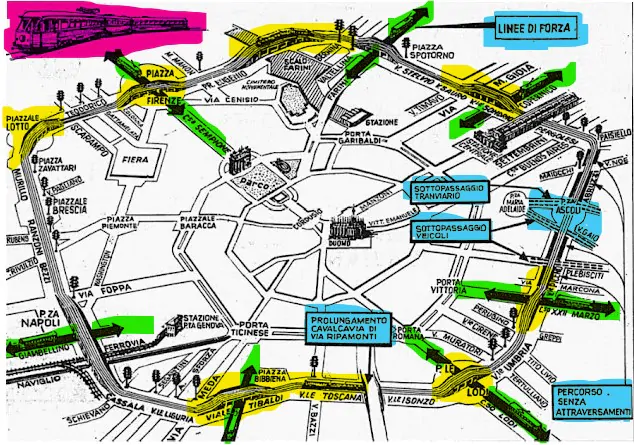
\includegraphics[width=1.0\textwidth]{figures/Milano-Circonvalla.png}
        \caption{Ring-Road of a Metropolitan City \cite{CorSera1973}}
      \end{figure}
    \end{column}
    \begin{column}{0.5\textwidth}
      \begin{figure}
        \centering
        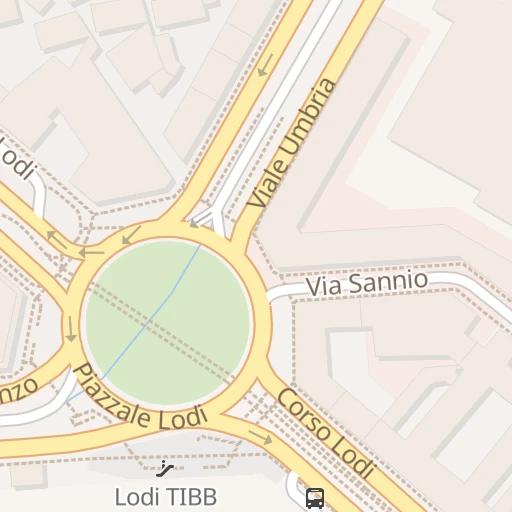
\includegraphics[width=1.00\textwidth]{figures/Milano-Intersezione.png}
        \caption{4-Way Double-Lane Traffic Light Regulated Intersection \cite{TuttoCitta2026}}
      \end{figure}
    \end{column}
  \end{columns}
\end{frame}

\begin{frame}
  \frametitle{The Multi-Agent Reinforcement Learning Story So Far}
  \begin{figure}
    \centering
    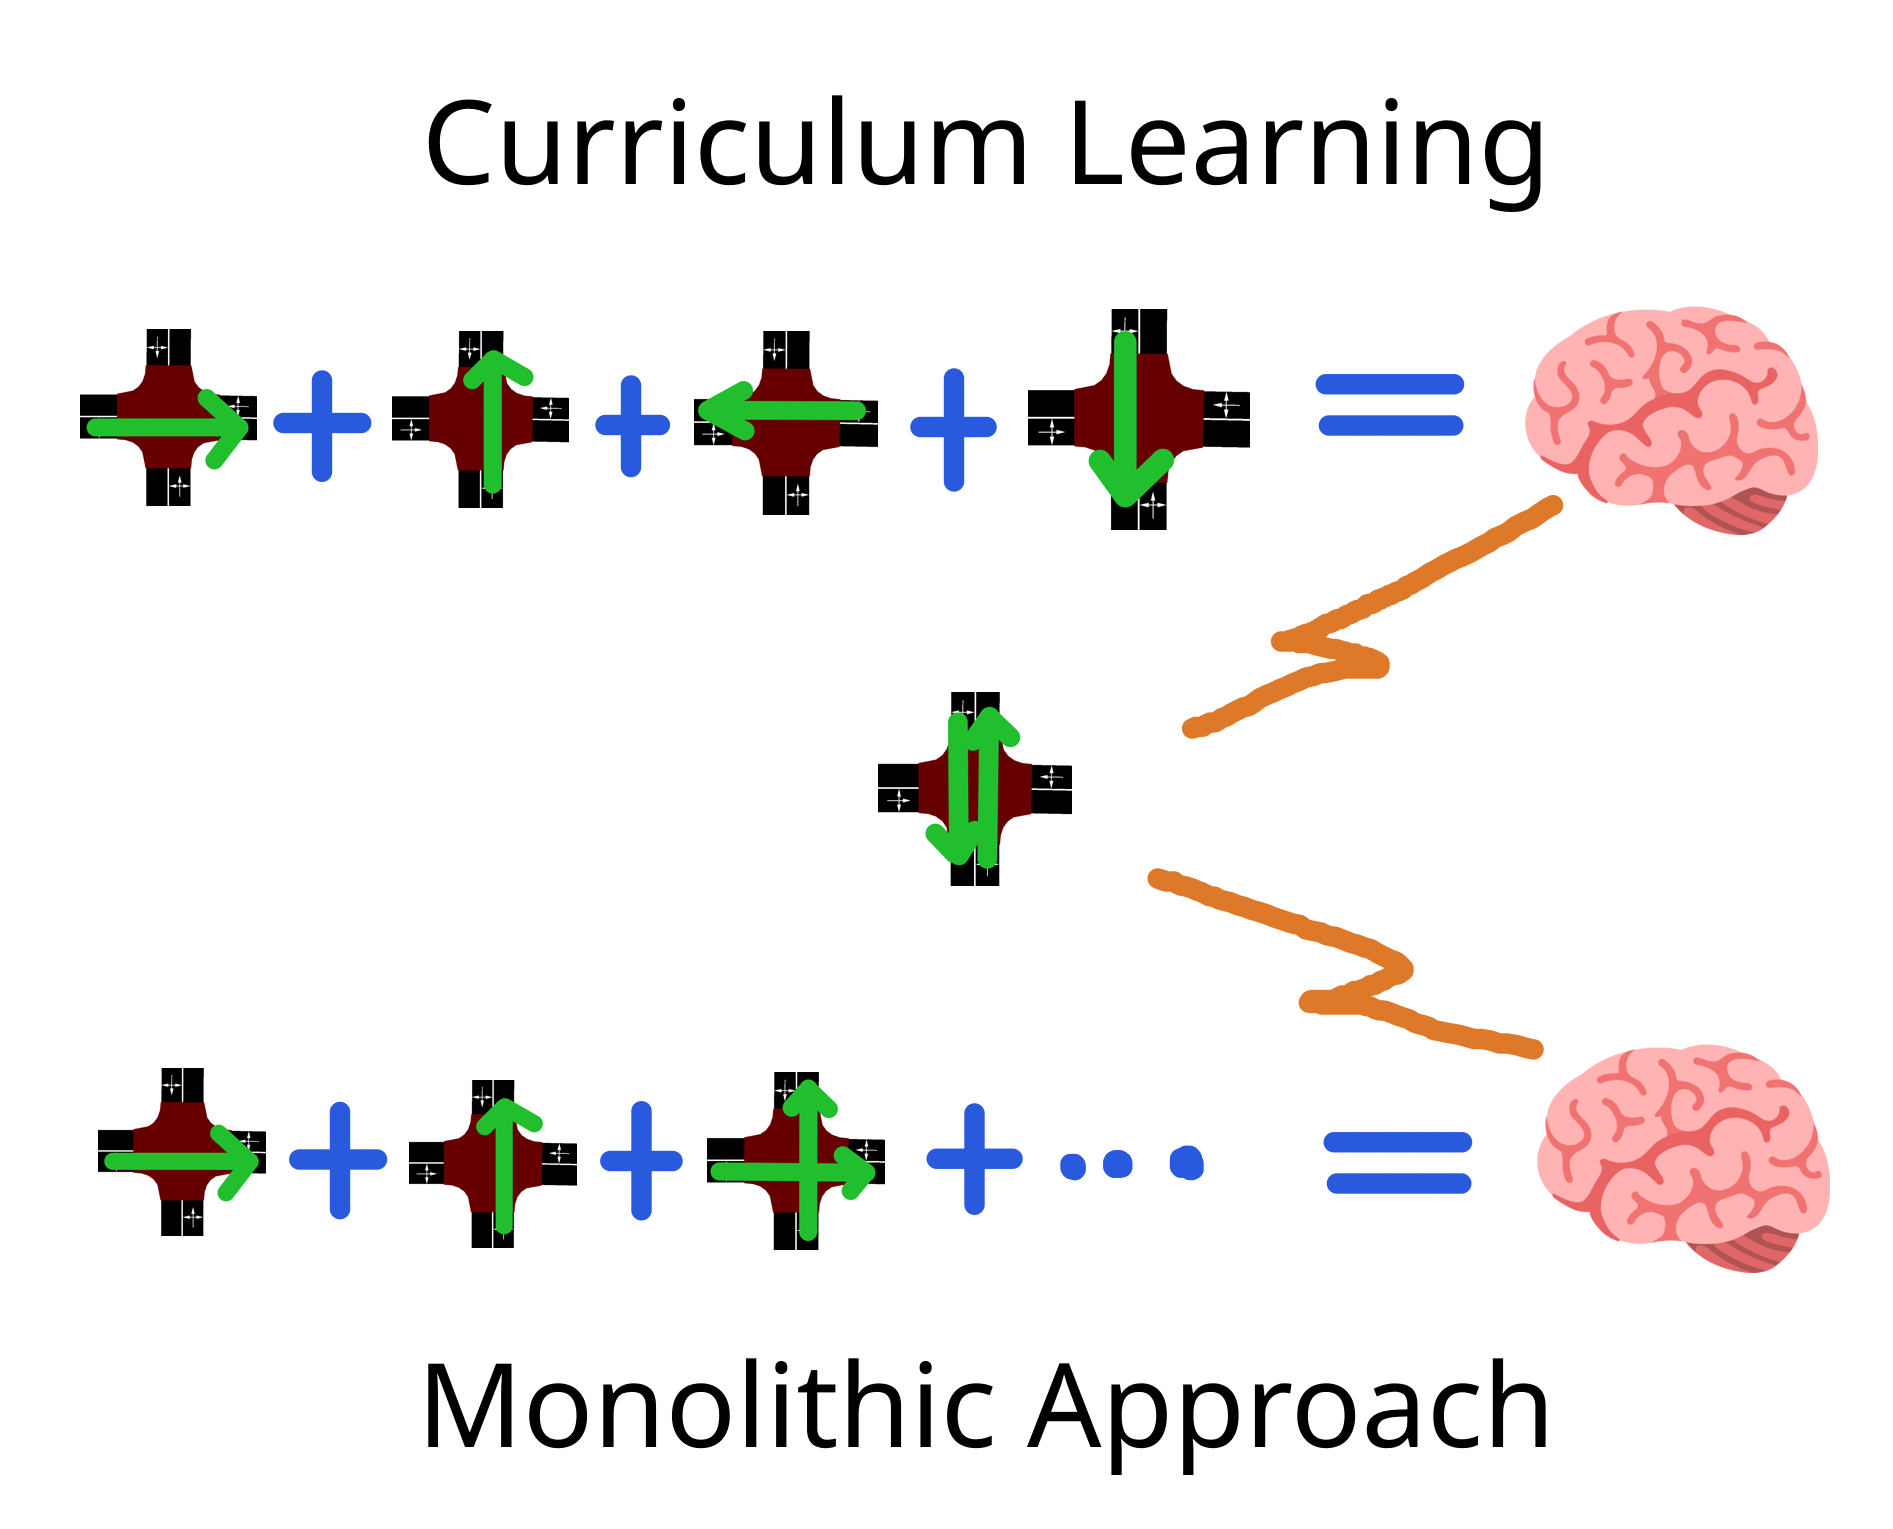
\includegraphics[width=0.65\textwidth]{figures/curriculum-vs-monolithic.png}
    \caption{Comparison of Approaches for Rearching Demand Coverage\cite{Refolli2025}}
  \end{figure}
\end{frame}

\begin{frame}
  \frametitle{The Multi-Agent Reinforcement Learning Story So Far}
  \begin{figure}
    \centering
    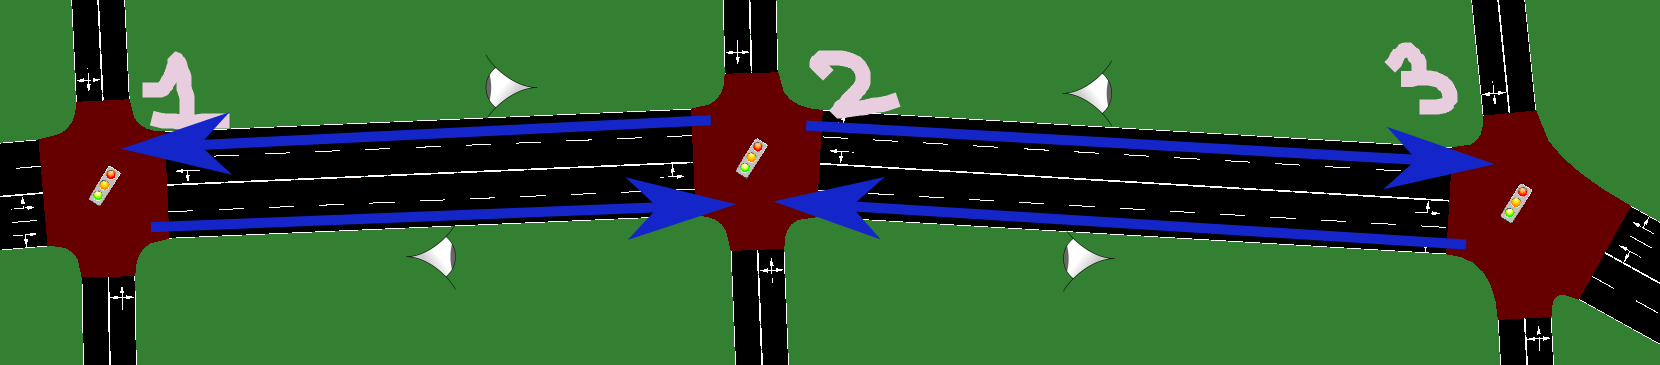
\includegraphics[width=0.75\textwidth]{figures/shared-observation-learning.png}
    \caption{Agents sharing Observation \cite{Refolli2025}}
  \end{figure}
  \begin{figure}
    \centering
    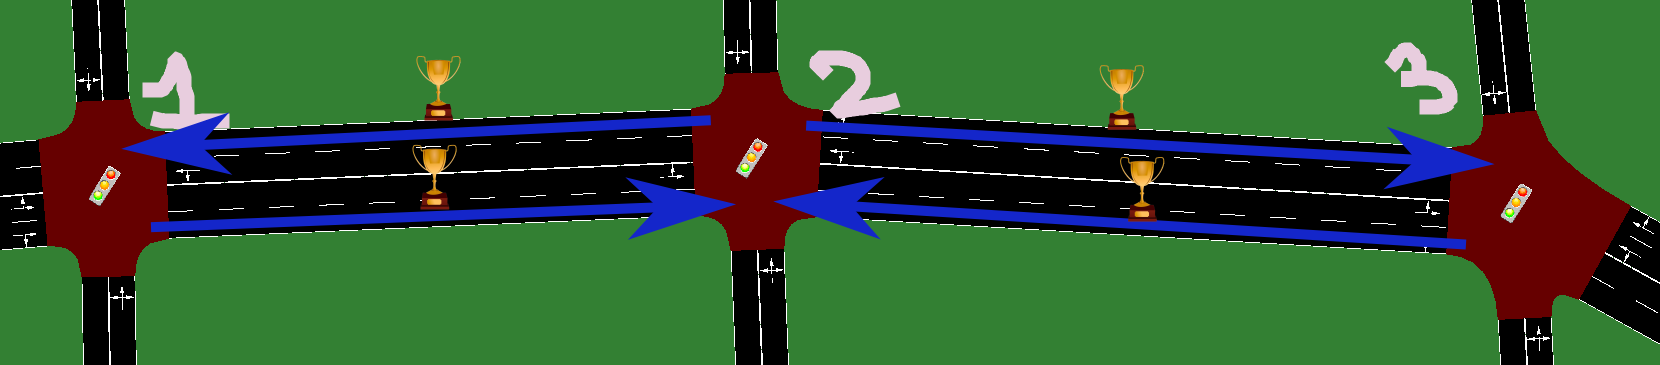
\includegraphics[width=0.75\textwidth]{figures/shared-reward-learning.png}
    \caption{Agents sharing Rewards \cite{Refolli2025}}
  \end{figure}
\end{frame}

\begin{frame}
  \frametitle{Centralized Reinforcement Learning}
  \begin{figure}
    \centering
    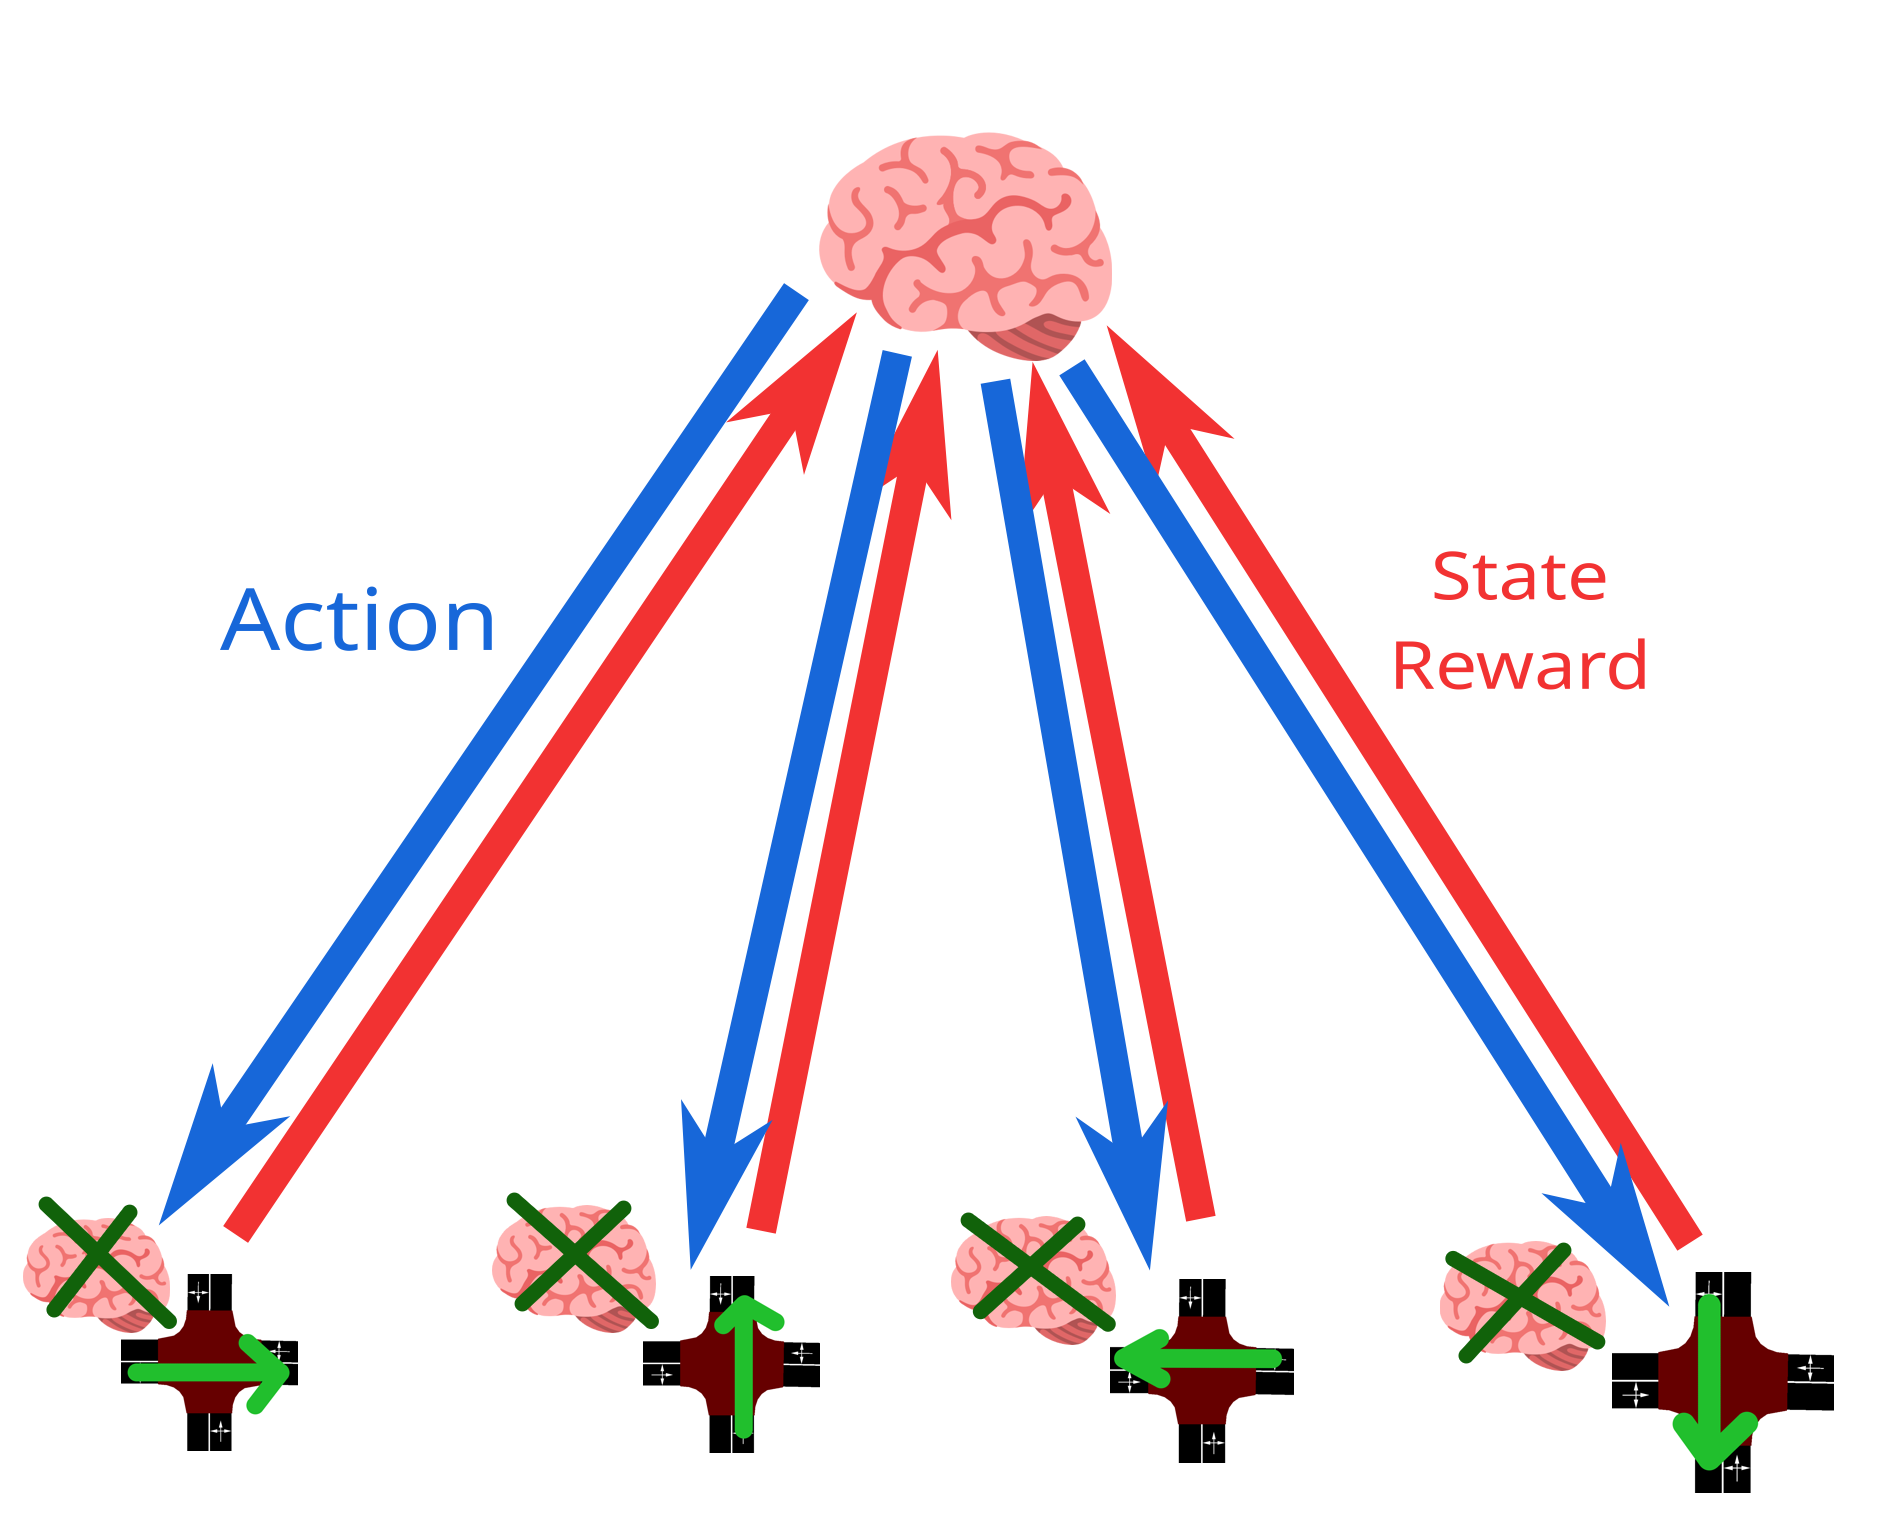
\includegraphics[width=0.75\textwidth]{figures/centralized-learning.png}
  \end{figure}
\end{frame}

\begin{frame}
  \frametitle{Federated Reinforcement Learning}
  \begin{figure}
    \centering
    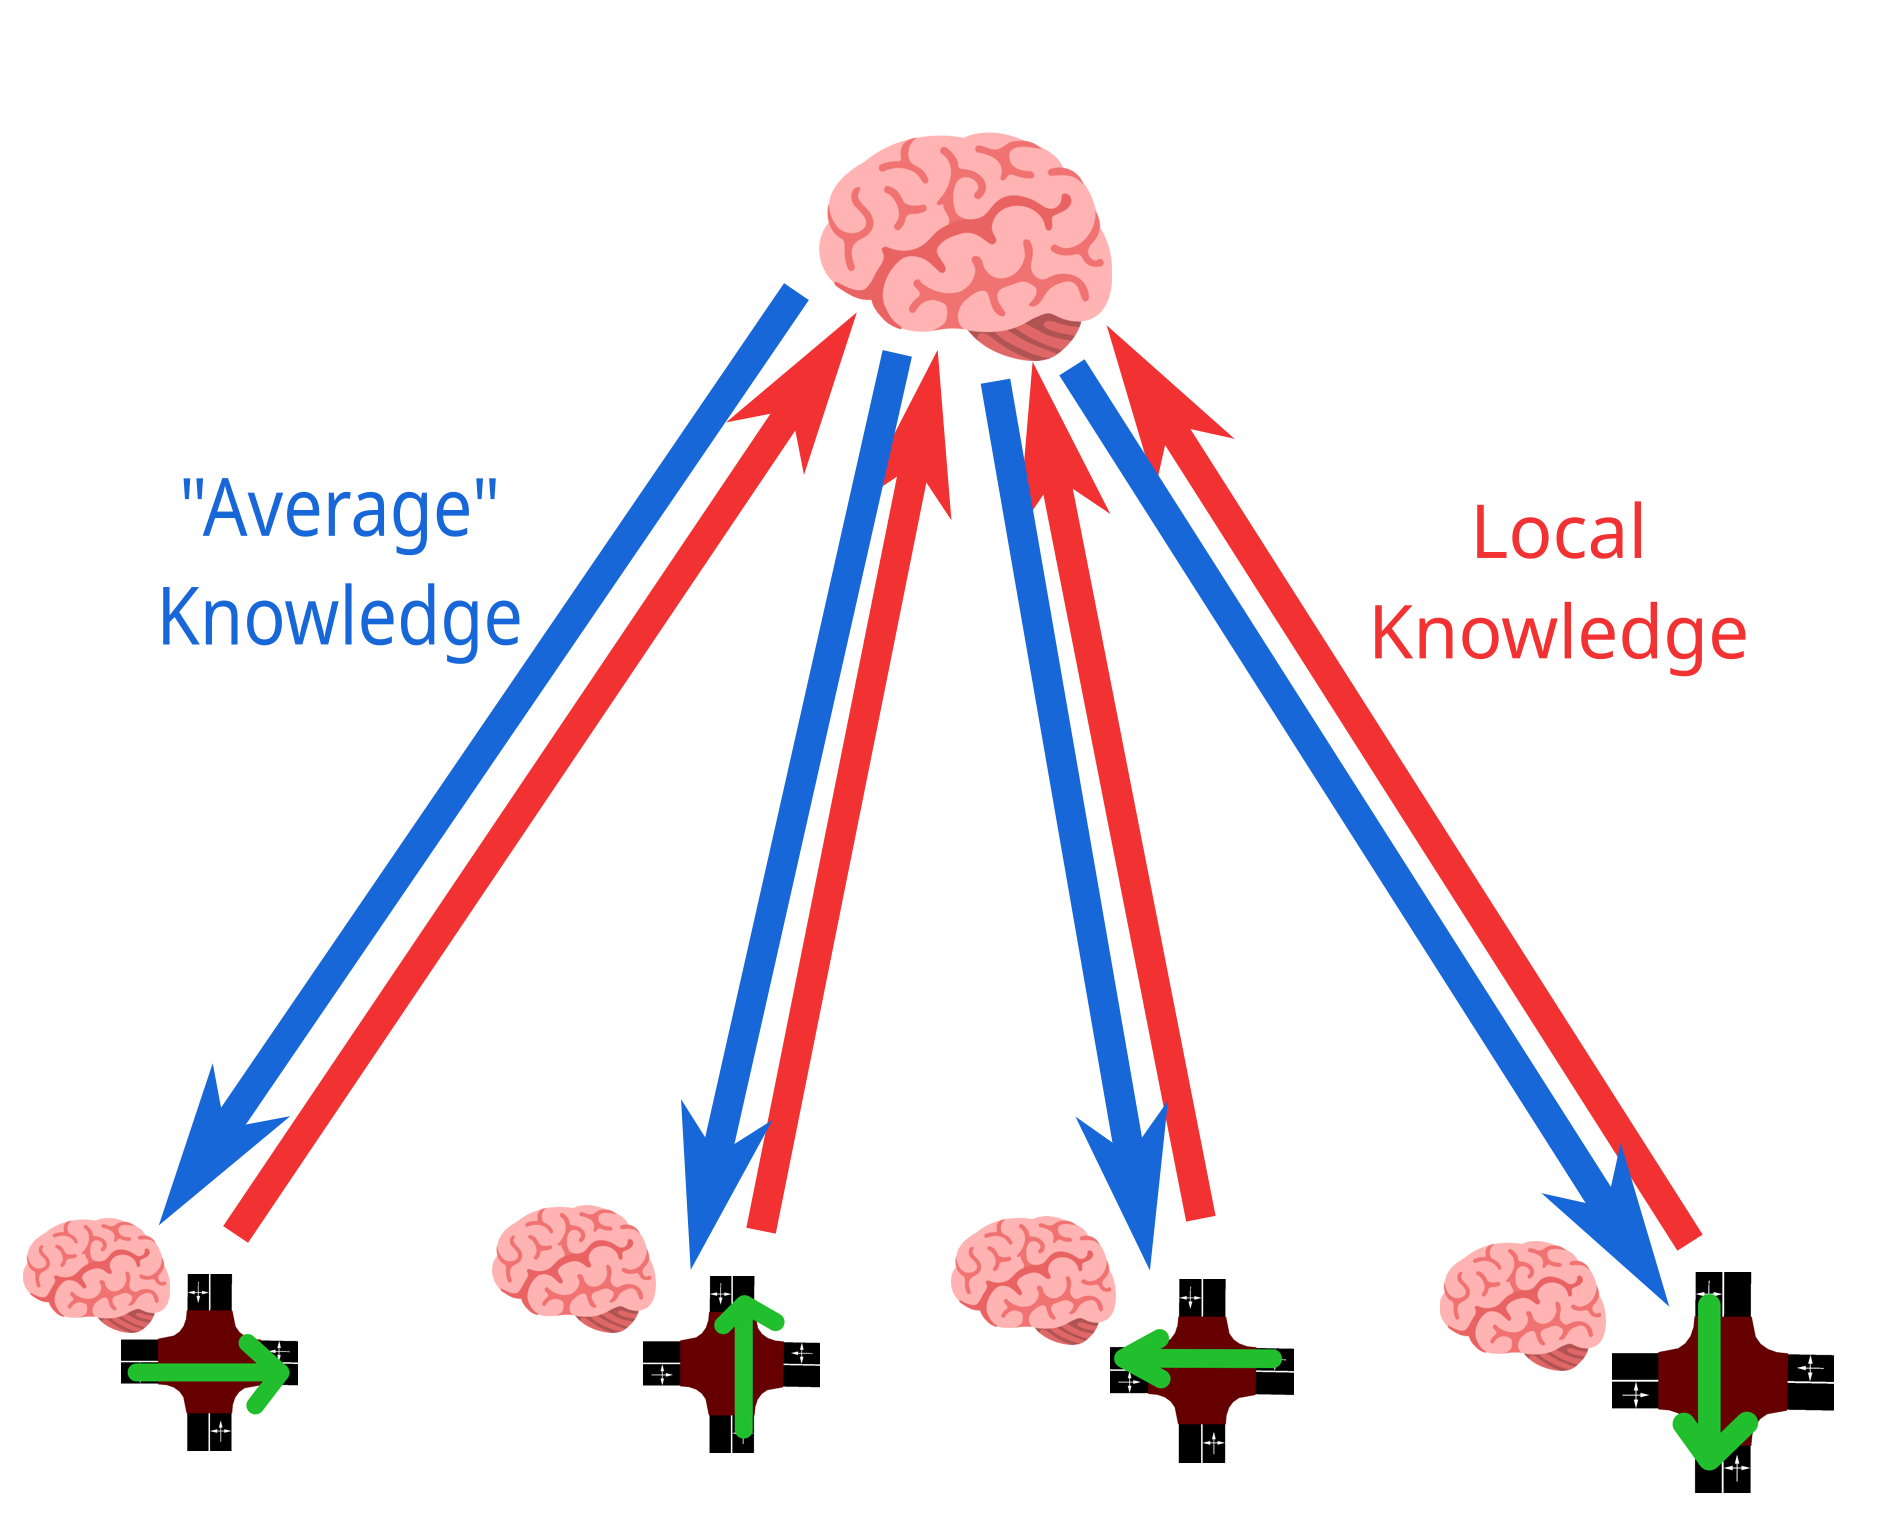
\includegraphics[width=0.75\textwidth]{figures/federated-learning.png}
  \end{figure}
\end{frame}

\begin{frame}
  \frametitle{The Simulator: UXsim}
  UXSim \cite{seo2025joss} is a Free and Open-Source \textit{macroscopic} and \textit{mesoscopic} network traffic flow simulator.
  It's tailored to simulate private-mobility simulations. It's \textbf{"Lightweight"}, \textbf{Library-Based} and \textbf{Written in Python}.
  \begin{columns}
    \begin{column}{0.5\textwidth}
      \begin{figure}
        \centering
        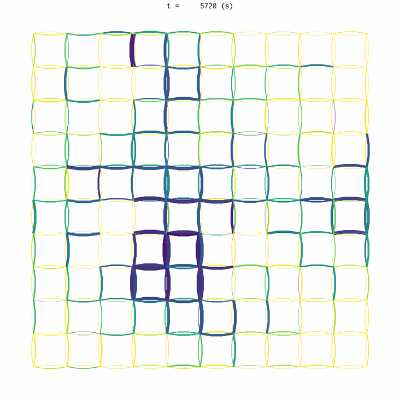
\includegraphics[width=0.8\textwidth]{figures/uxsim-example.png}
      \end{figure}
    \end{column}
    \begin{column}{0.5\textwidth}
      \begin{figure}
        \centering
        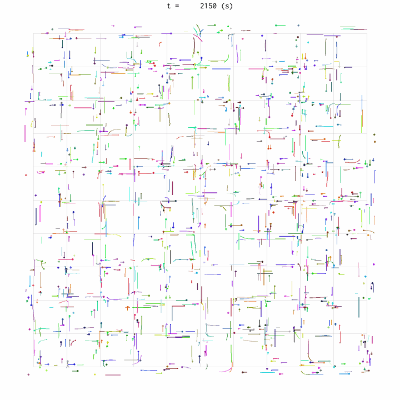
\includegraphics[width=0.8\textwidth]{figures/uxsim-example-2.png}
      \end{figure}
    \end{column}
  \end{columns}
\end{frame}

\begin{frame}
  \frametitle{The Agent Model}

  \begin{columns}
    \begin{column}{0.5\textwidth}
      \begin{itemize}
        \item The Agent can change Traffic Light Phase every 10 seconds
        \item Each one of the two \textit{phases} gives \textit{right of way} to one of the two flows
        \item The Agent can see the density of vehicles in each one of the roads (input/output)
        \item The Agent is rewarded based on vehicle queues' length, specifically on the amount vehicles en/dequeuing
      \end{itemize}
    \end{column}
    \begin{column}{0.5\textwidth}
      \begin{figure}
        \centering
        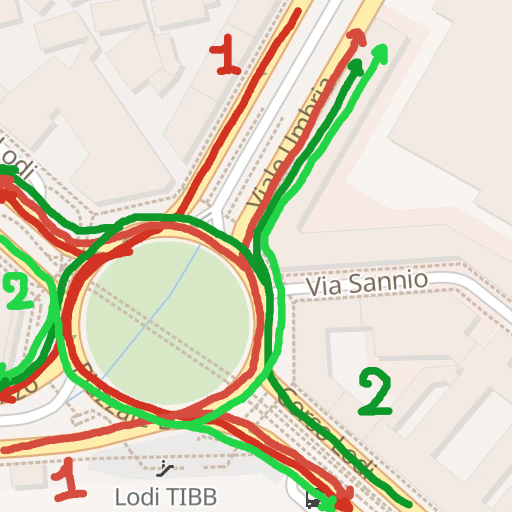
\includegraphics[width=1.0\textwidth]{figures/Milano-Agente.png}
        \caption{4-Way Double-Lane Traffic Light Regulated Intersection}
      \end{figure}
    \end{column}
  \end{columns}
\end{frame}

\begin{frame}
  \frametitle{The Traffic Model}

  \begin{columns}
    \begin{column}{0.5\textwidth}
      \begin{figure}
        \centering
        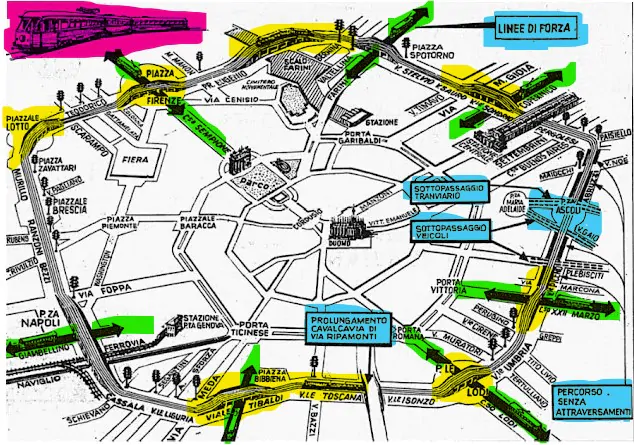
\includegraphics[width=1.0\textwidth]{figures/Milano-Circonvalla.png}
        \caption{Ring-Road of a Metropolitan City \cite{CorSera1973}}
      \end{figure}
    \end{column}
    \begin{column}{0.5\textwidth}
      \begin{itemize}
        \item Two-Lanes per Road Link
        \item Road Length is $1000$ m $=$ $1$ km
        \item Free Flow Speed is $20$ m/s $\approx$ $72$ km/h \cite{nagatani2002physics}
        \item Traffic Jam Density is set to $\rho = 0.2$ $\approx$ $40$ veh/2lanes/1km \cite{nagatani2002physics}
        \item No Platoons allowed, as in the Real-World (at least for now ...)
        \item No simulated Pedestrian Crossing, nor Public Transit (of any kind)
      \end{itemize}
    \end{column}
  \end{columns}
\end{frame}

\begin{frame}
  \frametitle{The Demand Model / Training Scenarios}

  \begin{columns}
    \begin{column}{0.5\textwidth}
      \begin{figure}
        \centering
        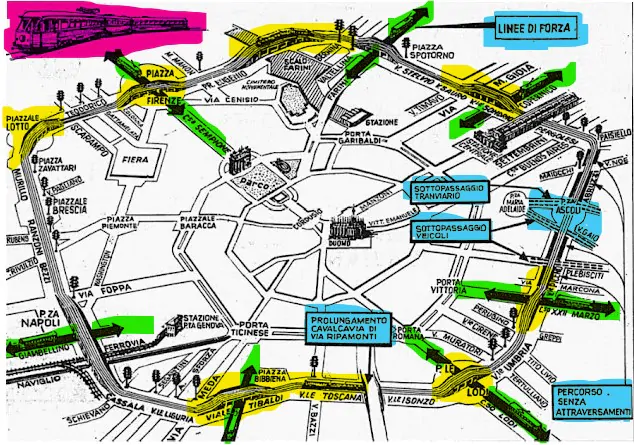
\includegraphics[width=1.0\textwidth]{figures/Milano-Circonvalla.png}
        \caption{Ring-Road of a Metropolitan City \cite{CorSera1973}}
      \end{figure}
    \end{column}
    \begin{column}{0.5\textwidth}
      \begin{itemize}
        \item All Mid \\
          (\textbf{Piazzale Fratelli Zavattari})
        \item Peak East to West \\
          (\textbf{Piazzale Loreto})
        \item Peak West to East \\
          (\textbf{Piazza Simone Bolivar})
        \item Peak North to South \\
          (\textbf{Piazza Firenze})
        \item Peak South to North \\
          (\textbf{Piazzale Lodi})
      \end{itemize}
    \end{column}
  \end{columns}
\end{frame}

\begin{frame}
  \frametitle{The Demand Model / Evaluation Scenarios}

  \begin{columns}
    \begin{column}{0.5\textwidth}
      \begin{figure}
        \centering
        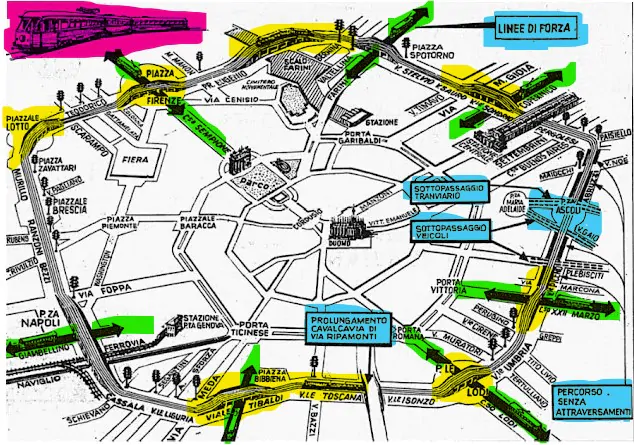
\includegraphics[width=1.0\textwidth]{figures/Milano-Circonvalla.png}
        \caption{Ring-Road of a Metropolitan City \cite{CorSera1973}}
      \end{figure}
    \end{column}
    \begin{column}{0.5\textwidth}
      \begin{itemize}
        \item Training Scenarios
        \item $+ \; 5 \; \times \;$ Random Demand
        \item Each entry of the four (EW, WE, NS, SN) is random
        \item Demand is in range $[0.3, 0.8]$
        \item The demand's percentage describes the amount of vehicles per unit of capacity
      \end{itemize}
    \end{column}
  \end{columns}
\end{frame}

\begin{frame}[fragile]
  \frametitle{The FedAvg Algorithm}

  \begin{columns}
    \begin{column}{0.5\textwidth}
      \begin{minipage}{\linewidth}
        \begin{lstlisting}[style=pythonstyle, caption=FedAvg Algorithm, mathescape]
def Coordinator():
  $\theta$ = Policy.New()
  $\forall c \in C \; | \; SendToClient(c, \theta)$
  for $e \in \{1,..,E\}$:
    $\{(\theta_1, w_1) ...\} = \{ GetFromClient(c) \; | \; \forall c \in C\}$
    $\{\alpha_1 ...\} = \{\frac {w_1} {\Sigma w_i} ...\}$
    $\theta = \Sigma \alpha_i \theta_i$
    $\forall c \in C \; | \; SendToClient(c, \theta)$
  return $\theta$

def Client(scenario):
  for $e \in \{1,..,E\}$:
    $\theta = GetFromCoordinator()$
    $\theta', w$ = Simulation($\theta$, scenario)
    $SendToCoordinator(\theta')$
        \end{lstlisting}
      \end{minipage}
    \end{column}
    \begin{column}{0.5\textwidth}
      \begin{itemize}
        \item Knowledge is weighted on the complexity of the scenario of a client
        \item ... which is equal to the demand that the client has to deal with
        \item Due to resource constrains, only 5 Peers were used, with no client sampling
        \item The duration of a simulation is $3600s \; = \; 1hr \; = \; 360$ steps.
      \end{itemize}
    \end{column}
  \end{columns}
\end{frame}

\begin{frame}
  \frametitle{Results / Training}
  \begin{figure}
    \centering
    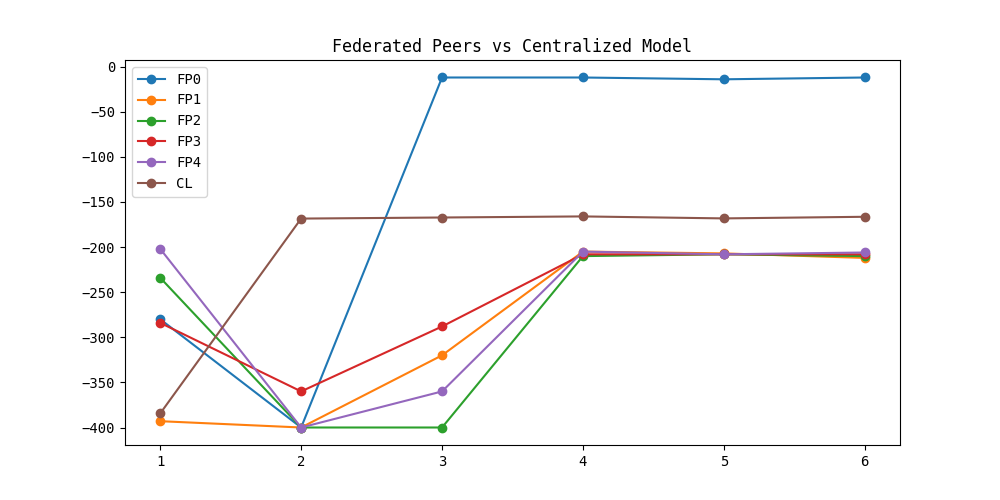
\includegraphics[width=\textwidth]{figures/models-training-stats.png}
    \caption{Total Reward during Training over Time (Episodes)}
  \end{figure}
\end{frame}

\begin{frame}
  \frametitle{Results / Evaluation}
  \begin{figure}
    \centering
    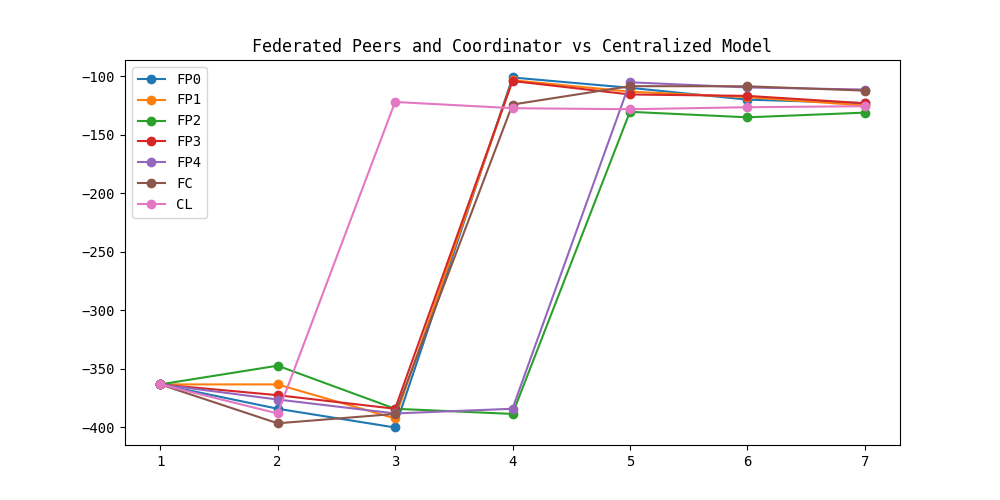
\includegraphics[width=\textwidth]{figures/models-evaluation-stats.png}
    \caption{Average Total Reward during Evaluation over Time (Initial + Episodes)}
  \end{figure}
\end{frame}

\begin{frame}
  \frametitle{Results / The Federated Coordinator is Catching Up!}
  \begin{figure}
    \centering
    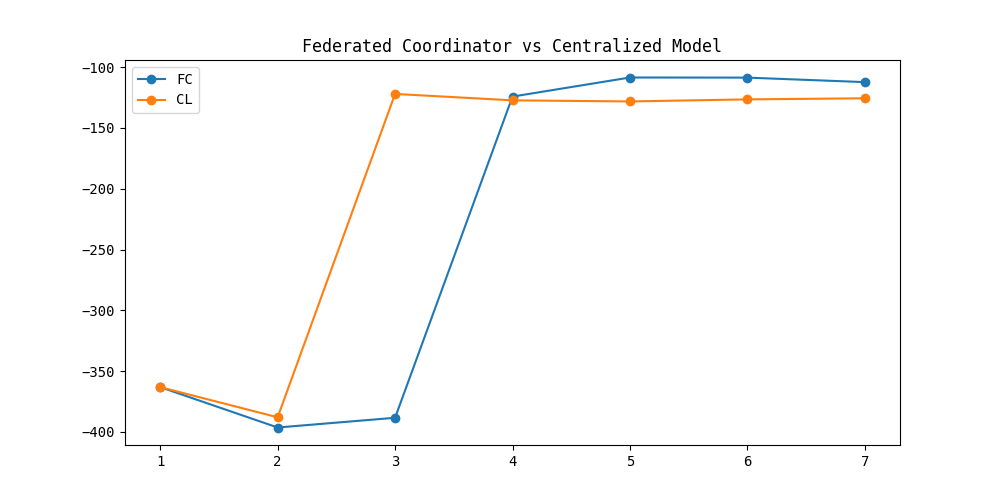
\includegraphics[width=\textwidth]{figures/federated-coordinator-catching-up.png}
    \caption{Average Total Reward during Evaluation over Time (Initial + Episodes)}
  \end{figure}
\end{frame}

\begin{frame}
  \frametitle{Comparisons / Fixed-Cycle Agents}
  \begin{figure}
    \centering
    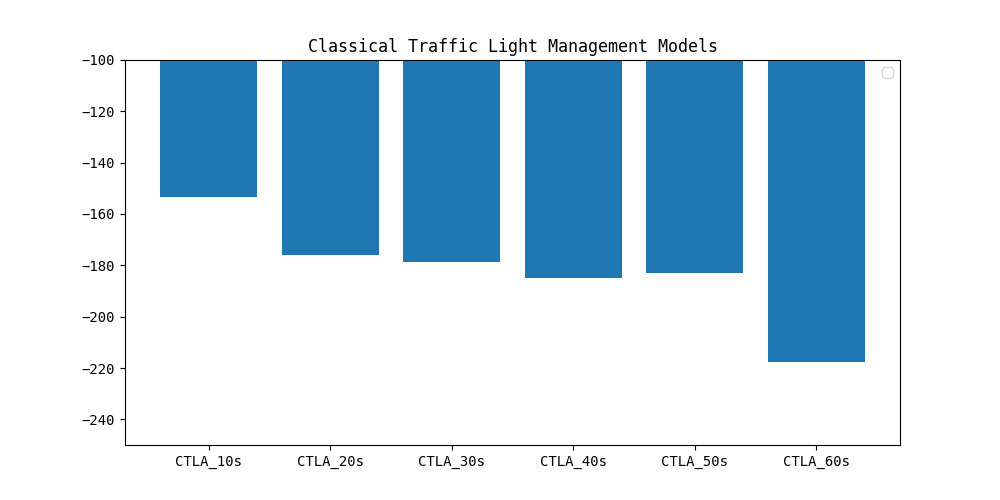
\includegraphics[width=\textwidth]{figures/CTLA-10-is-best-60-is-worst.png}
    \caption{Average Total Reward during Evaluation of Fixed-Cycle Agents (\textit{CTLA\_Ts} means $T$ seconds per phase)}
  \end{figure}
\end{frame}

\begin{frame}
  \frametitle{Comparisons / Is Deep Q-Learning Worth the Effort?}
  \begin{figure}
    \centering
    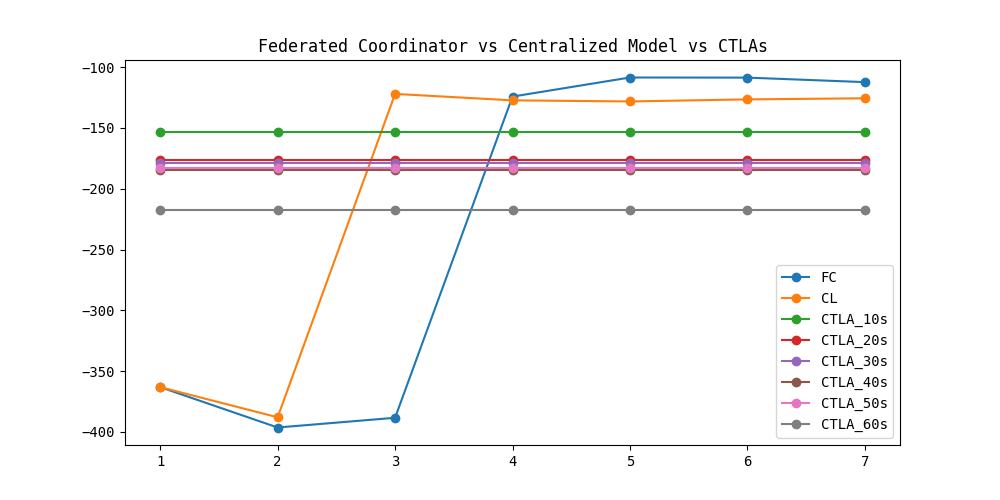
\includegraphics[width=\textwidth]{figures/FedRL-and-CRL-Learned-a-Better-Policy-then-CTLA.png}
    \caption{Comparison of Average Total Reward obtained by Deep Q-Learning Models and Fixed-Cycle Agents during Evaluation}
  \end{figure}
\end{frame}

\begin{frame}
  \frametitle{Comparisons / Is Deep Q-Learning Worth the Effort?}
  \begin{figure}
    \centering
    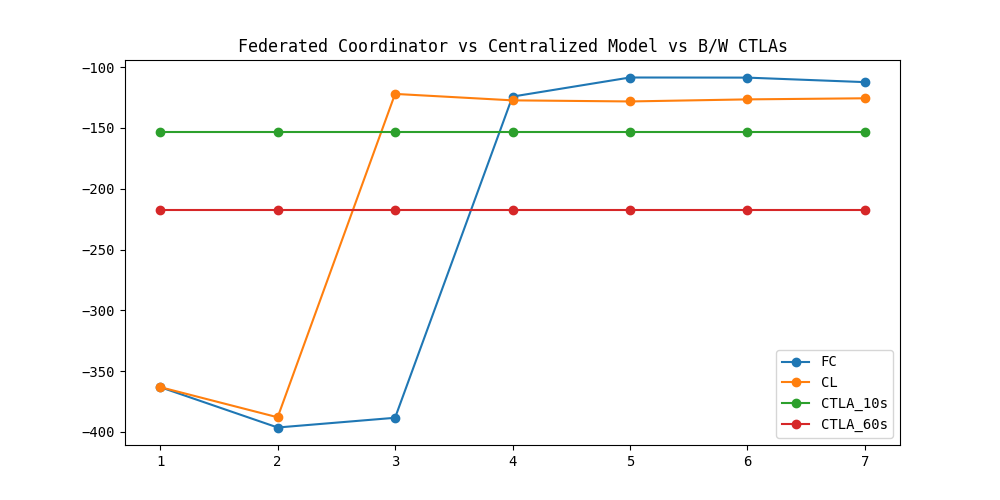
\includegraphics[width=\textwidth]{figures/FedRL-and-CRL-Learned-a-Better-Policy-then-B_W_CTLA.png}
    \caption{Comparison of Average Total Reward obtained by Deep Q-Learning Models and Fixed-Cycle Agents during Evaluation}
  \end{figure}
\end{frame}

\begin{frame}
  \frametitle{Visualizing that Reward Difference}
  \begin{columns}
    \begin{column}{0.5\textwidth}
      \begin{figure}
        \centering
        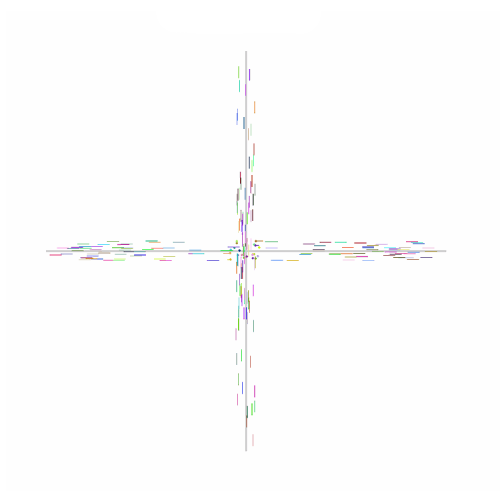
\includegraphics[width=1.0\textwidth]{figures/gif-CTLA-10s.png}
        \caption{Microscopic visualization of Fixed-Agent (10s per phase)}
      \end{figure}
    \end{column}
    \begin{column}{0.5\textwidth}
      \begin{figure}
        \centering
        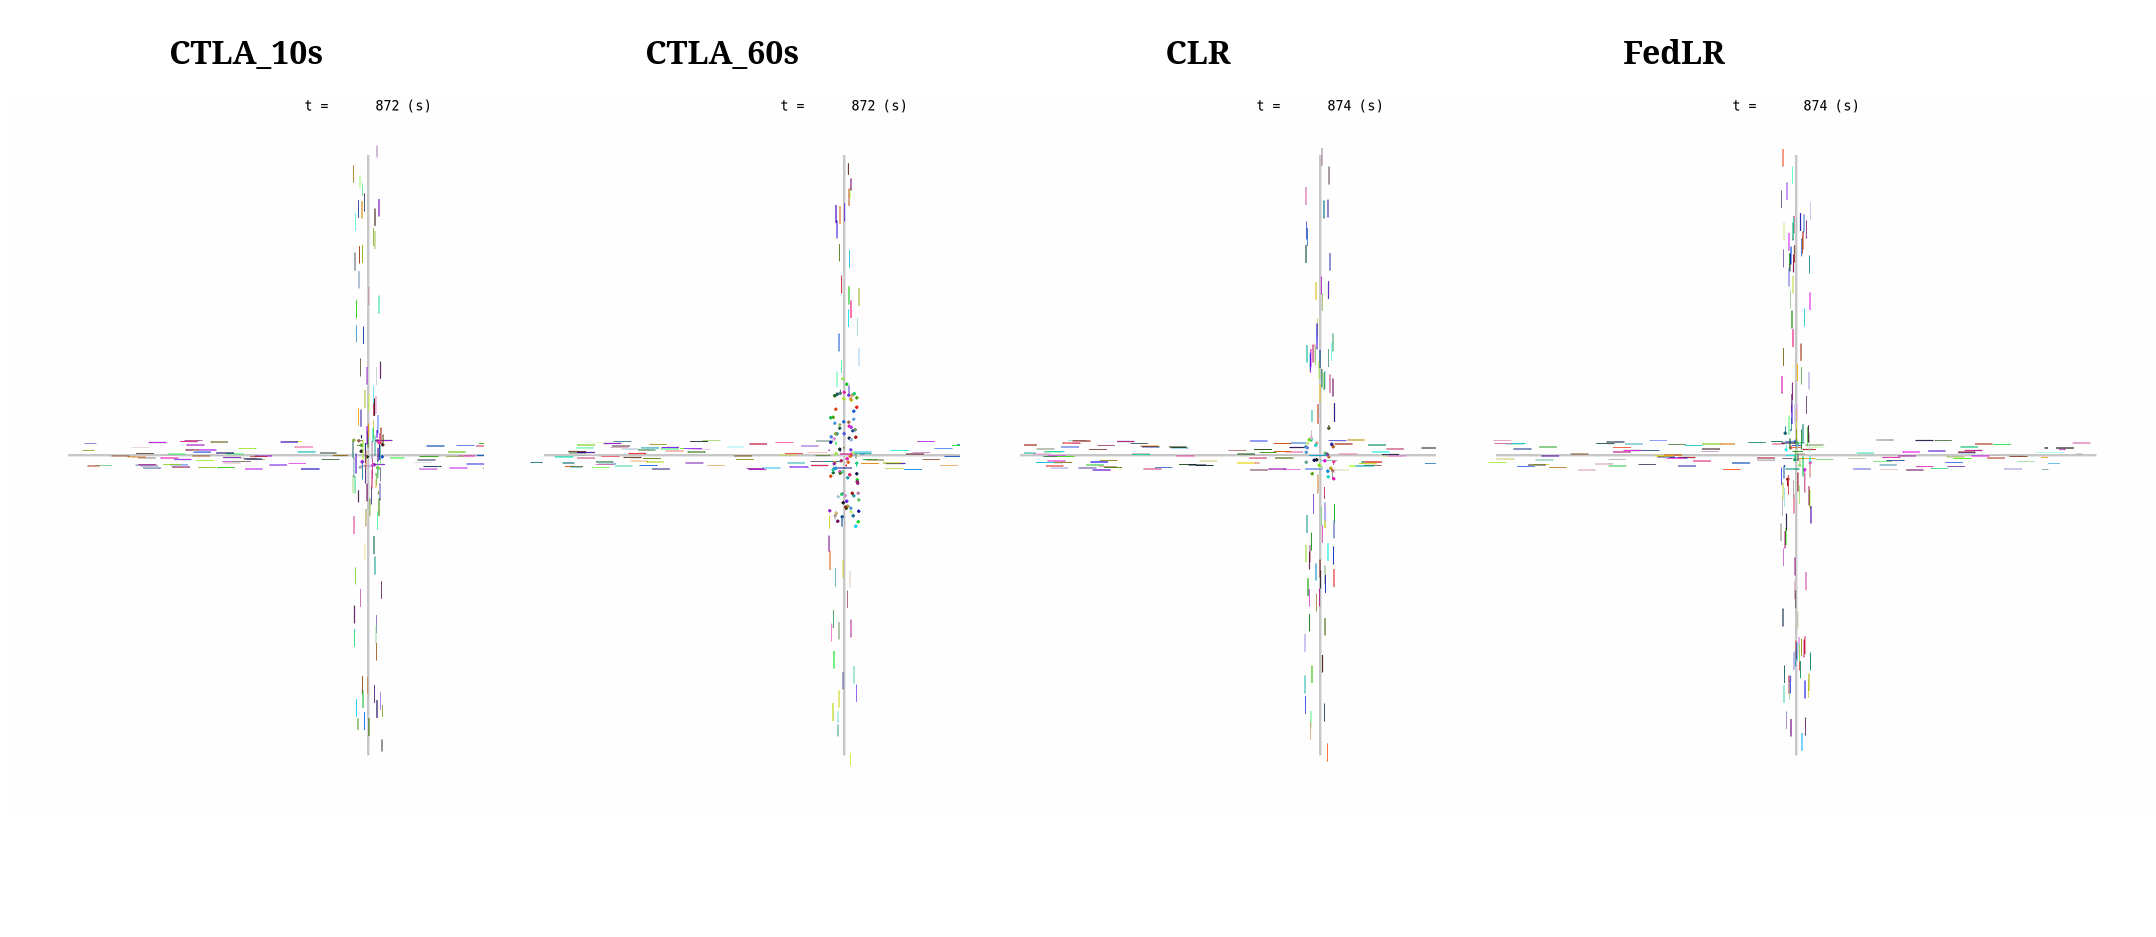
\includegraphics[width=1.0\textwidth]{figures/gif-CTLA-60s.png}
        \caption{Microscopic visualization of Fixed-Agent (60s per phase)}
      \end{figure}
    \end{column}
  \end{columns}
\end{frame}

\begin{frame}
  \frametitle{Visualizing that Reward Difference}
  \begin{columns}
    \begin{column}{0.5\textwidth}
      \begin{figure}
        \centering
        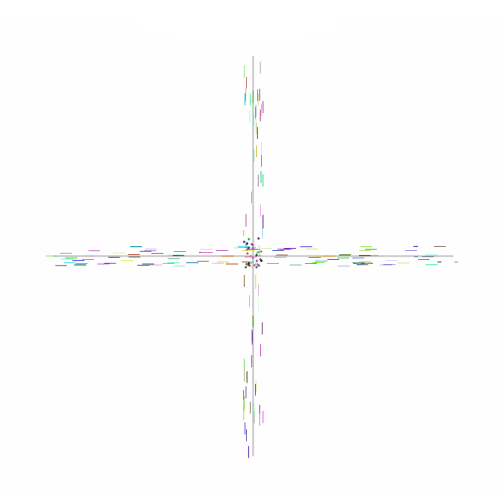
\includegraphics[width=1.0\textwidth]{figures/gif-CLR.png}
        \caption{Microscopic visualization of Centralized Learning Agent}
      \end{figure}
    \end{column}
    \begin{column}{0.5\textwidth}
      \begin{figure}
        \centering
        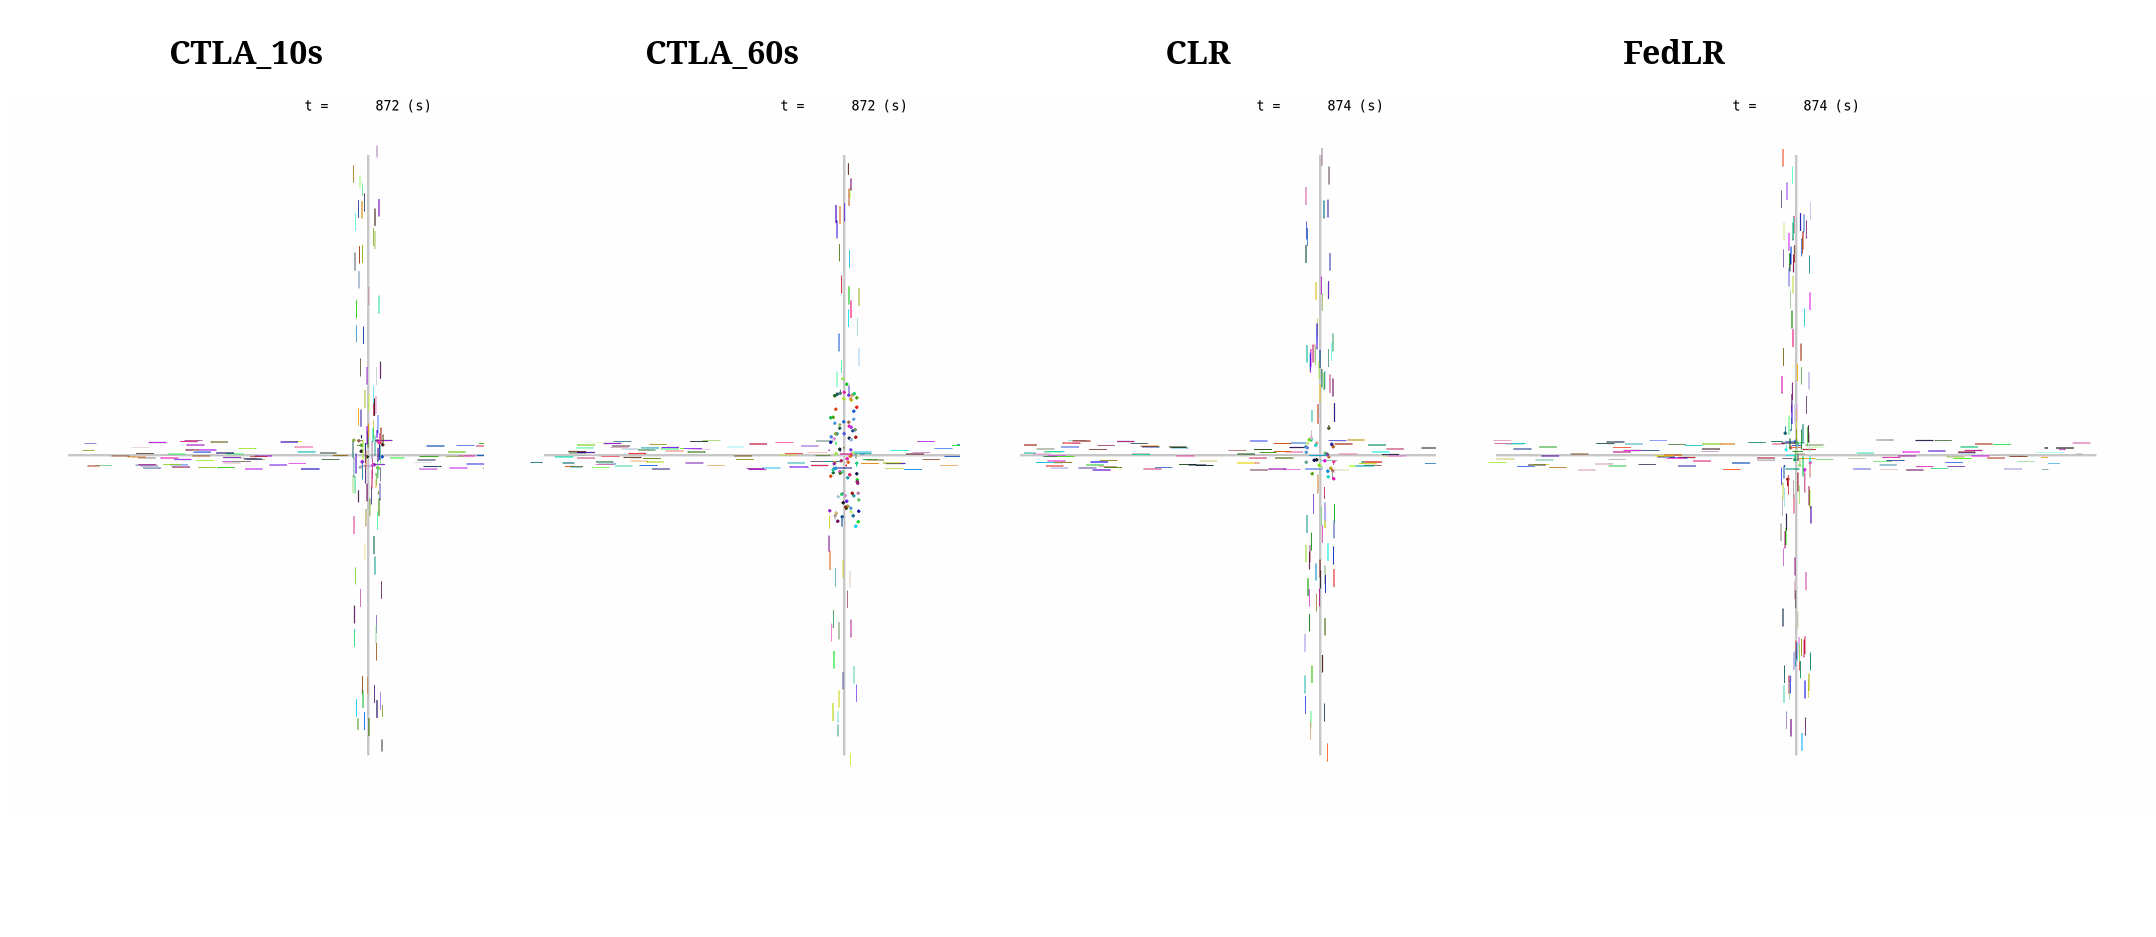
\includegraphics[width=1.0\textwidth]{figures/gif-FedLR.png}
        \caption{Microscopic visualization of Federated Learning Agent}
      \end{figure}
    \end{column}
  \end{columns}
\end{frame}

\begin{frame}
  \centering
  \Huge
  Thank You
%\cite{Refolli2025}
  \begin{figure}
    \centering
    %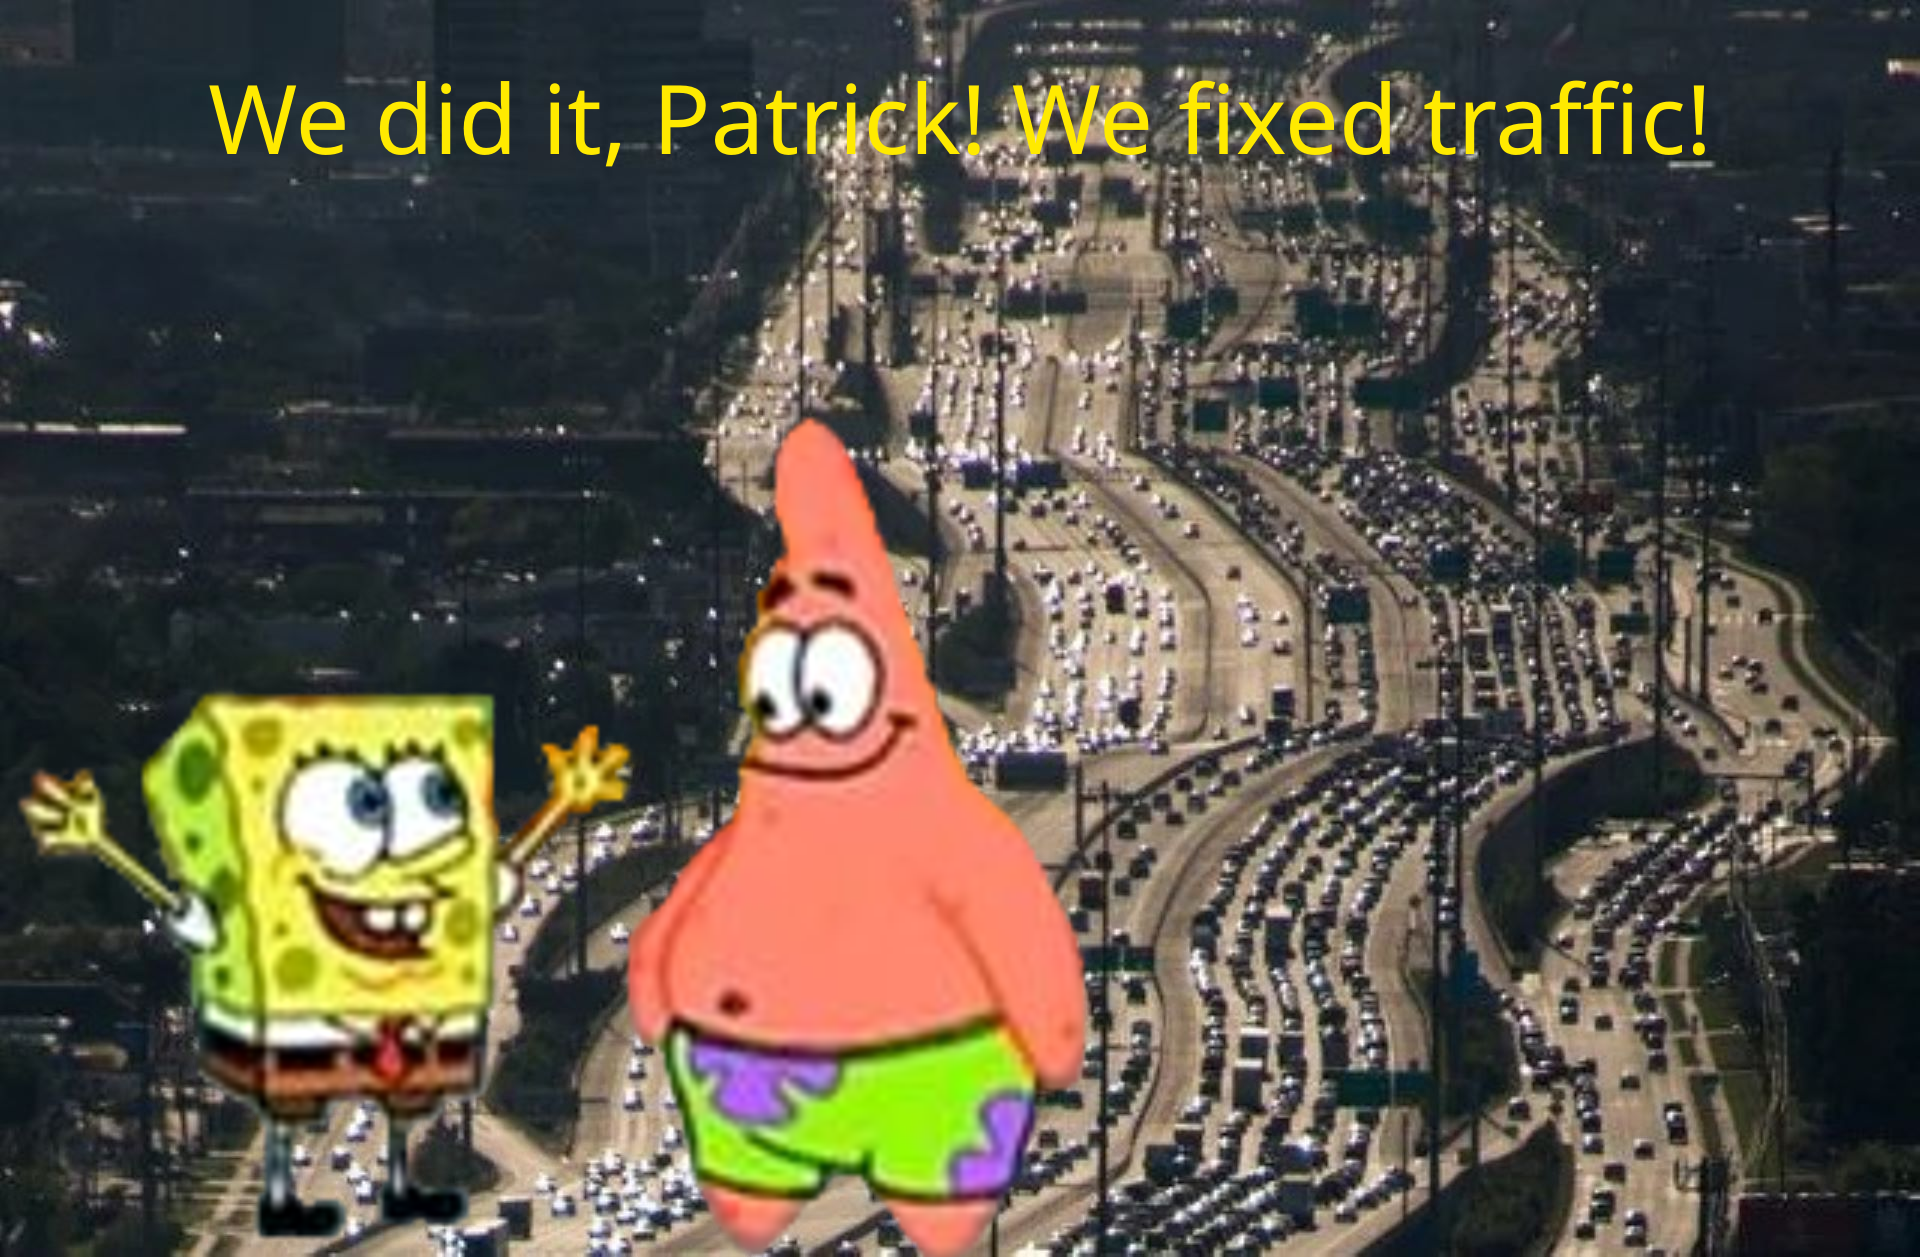
\includegraphics[width=0.9\textwidth]{figures/patrick.png}
    
\includegraphics[width=0.9\textwidth]{figures/github-repo.png}
  \end{figure}
\end{frame}

\begin{frame}[allowframebreaks, noframenumbering]
\frametitle{Bibliography}
\printbibliography
\nocite{*}
\end{frame}

\end{document}
